\section{Naive Bayes Classifiers}

Another family of supervised learning models that's related to linear classification models is the Naive Bayes family of classifiers, which are based on simple \emph{probabilistic} models of how the data in each class might have been generated. 

Naive Bayes classifiers are called naive because informally, they make the \emph{simplifying assumption} that each feature of an instance is independent of all the others, given the class. 

In practice, of course, this is not often the case, features often are somewhat correlated. For example, in predicting whether a house is likely to sell above the owner's asking price. Some features, such as the are of the interior rooms are likely to be correlated with other features, such as the size of the land that the house is built on or the number of bedrooms. And these features in turn might be correlated with the location of the property, and so on. 

This naive simplifying assumption means on the one hand, that learning a Naive Bayes classifier is \emph{very fast}. Because only simple per class statistics need to be estimated for each feature and applied for each feature independently. 

On the other hand, the penalty for this efficiency is that the \emph{generalization performance} of Naive Bayes Classifiers can often be a bit worse than other more sophisticated methods, or even linear models for classification. 

Even so, especially for high dimensional data sets, Naive Bayes Classifiers can achieve \emph{performance} that's often competitive to other more sophisticated methods, like support vector machines, for some tasks. 

There are three flavors of Naive Bayes Classifier that are available in scikit learn.

\subsection{Bernoulli Naive Bayes model}

The Bernoulli Naive Bayes model uses a set of \emph{binary} occurrence features. When classifying texts document for example, the Bernoulli Naive Bayes model is quit handy because we could represent the presence or the absence of the given word in the text with the binary feature. 

Of course this doesn't take into account how often the word occurs in the text. 

\subsection{Multinomial Naive Bayes model}

So the Multinomial Naive Bayes model uses a set of count base \emph{discrete} features each of which does account for how many times a particular feature such as a word is observed in training example like a document. 

In this lecture we won't have time to cover the Bernoulli or Multinomial Naive Bayes models. However, those models are particularly well suited to textual data, where each feature corresponds to an observation for a particular word. And so you'll see Naive Bayes again, including the Bernoulli and Multinomial models in more depth in the text mining part of this specialization. 

\subsection{Gaussian Naive Bayes model}

This lecture will focus on Gaussian Naive Bayes classifiers which assume features that are \emph{continuous or real-valued}. During training, the Gaussian Naive Bayes Classifier estimates for each feature the \texttt{mean} and \texttt{standard deviation} of the feature value for each class. 

For prediction, the classifier compares the features of the example data point to be predicted with the feature statistics for each class and selects the class that best matches the data point. 

More specifically, the Gaussian Naive Bayes Classifier assumes that the data for each class was generated by a simple class specific \emph{Gaussian distribution}. 

Predicting the class of a new data point corresponds mathematically to estimating the probability that each classes Gaussian distribution was most likely to have generated the data point. Classifier then picks the class that has the highest probability. 

Without going into the mathematics involved, it can be shown that the decision boundary between classes in the two class Gaussian Naive Bayes Classifier. In general is a \emph{parabolic} curve between the classes. 

And in the special case where the variance of these feature is the same for both classes. The decision boundary will be linear. 

Here's what that looks like, typically, on a simple binary classification data set. 

The gray ellipses given idea of the shape of the Gaussian distribution for each class, as if we were looking down from above. 

You can see the centers of the Gaussian's correspond to the mean value of each feature for each class. 

More specifically, the gray ellipses show the contour line of the Gaussian distribution for each class, that corresponds to about two standard deviations from the mean. 

\begin{center}
	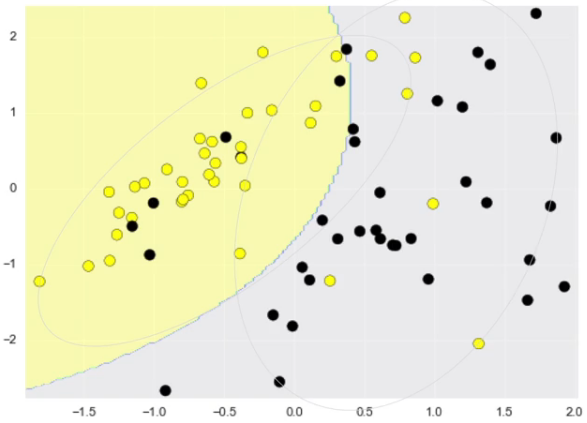
\includegraphics[width=\linewidth]{img/Gaussian-Naive-Bayes-Classifier-1.png} 
\end{center}


The line between the yellow and gray background areas represents the decision boundary. And we can see that this is indeed parabolic. 

To use the Gaussian Naive Bayes classifier in Python, 
we just instantiate an instance of the Gaussian NB class and call the fit method on the training data just as we would with any other classifier. 

\begin{verbatim}
from sklearn.naive_bayes import GaussianNB
\end{verbatim}

\textbf{Note:} the Naive Bayes models are among a few classifiers in scikit learn that support a method called \texttt{partial_fit},  which can be used instead of \texttt{fit} to train the classifier \emph{incrementally} in case you're working with a huge data set that doesn't fit into memory. 

For the \texttt{GaussianNB} class there are no special parameters to control the models complexity. 

Looking at one example in the notebook from our synthetic two class dataset, we can see that, in fact, the Gaussian Naive Bayes classifier achieves quite good performance on this simple classification example. When the classes are no longer as easily separable as with this second, more difficult binary example here. Like linear models, Naive Bayes does not perform as well. 

On a real world example, using the breast cancer data set, the Gaussian Naive Bayes Classifier also does quite well, being quite competitive with other methods, such as support vector classifiers. 

{\scriptsize
\begin{verbatim}
X_train, X_test, y_train, y_test = 
train_test_split(X_cancer, y_cancer, random_state = 0)

nbclf = GaussianNB().fit(X_train, y_train)
print('Breast cancer dataset')
print('Accuracy of GaussianNB classifier on training 
  set: {:.2f}'.format(nbclf.score(X_train, y_train)))
print('Accuracy of GaussianNB classifier on test set:
 {:.2f}'.format(nbclf.score(X_test, y_test)))

Breast cancer dataset
Accuracy of GaussianNB classifier on training set: 0.95
Accuracy of GaussianNB classifier on test set: 0.94
\end{verbatim}
}

Typically, Gaussian Naive Bayes is used for \emph{high-dimensional} data, when each data instance has hundreds, thousands or maybe even more features. Likewise the Bernoulli and Nultinomial flavors of Naive Bayes are used for text classification where there are very large number of distinct words is features and where the future vectors are sparse because any given document uses only a small fraction of the overall vocabulary. 

The Naive Bayes Classifiers are related mathematically to linear models, so many of the pros and cons of linear models also apply to Naive Bayes. 

On the \textbf{positive} side Naive Bayes classifiers are:
\begin{itemize}
\item easy to understand;
\item fast to train and use for prediction;
\item well suitable to high dimensional data including text and the applications involving very large data sets, where efficiency is critical and computational costs rule out other classification approaches;
\item often useful as a baseline comparison against more sophisticated methods.
\end{itemize}


On the \textbf{negative} side:
\begin{itemize}
\item assumption that features are conditionally independence are not realistic; for many real world datasets there's significant covariance among features;
\item other classifier types often have better generalization performance;
\item confidence estimates for predictions are not very accurate.
\end{itemize}

Other more sophisticated classification methods that can account for these dependencies are likely to outperform Naive Bayes. 

And on a side note, when getting confidence or probability estimates associated with predictions, Naive Bayes classifiers produce unreliable estimates, typically. 

Still, Naive Bayes Classifiers can perform very competitively on some tasks, and are also often very useful as baseline models against which more sophisticated models can be compared. 